\subsection{Digital Topology}
\label{sec:digital-topology}

In two dimensions, a black and white image consists of an array of pixels
where each pixel is either black or white.
This idea can be extended to three dimensions,
instead of square pixels we have cubes called voxels.
Three dimensional images are use useful in medical images. 
For example,  consider a
three dimensional images of the human heart \cite{bovik_handbook_2000}.
Given such an image, one might want to compute
the number of holes in the image to make sure it
matches the number of holes that are suppose to be in
the human heart. In this subsection, we share a result
of Chen and Rong where they 
use the Gauss-Bonnet theorem to 
compute genus of a digital image in $\R^3$ \cite{chen_digital_2010}.


Digital images are commonly reffered to as \emph{cubical complexes},
where each cube has side length one \cite{kong_digital_1989}.
An \emph{elementary cube} $Q$ is a product
$$Q=I_1\times I_2 \times I_3$$
where each $I_i$ is a unit interval of the form $I=[\ell,\ell+1]$
called a \emph{coordinate}.
We will often associate each elementary cube with a lattice point
see \figref{4-square-and-dual} for an example.
%In many cases, given a cubical complex, one is interested in having
%a computer to to classify the image.
%Operations toward image classification include
%object counting, border following and computing 
%the number of holes \cite{kong_digital_1989}.


In two dimensions, it is not clear what it means
for two pixels to be adjacent. For example, in \figref{4-square}
we see four black pixels. Should these pixels represent a closed
curve? If we define the pixels adjacent to a given pixel to be the 
pixels to the left, right, above, and below, then each black pixel isolated
and the four pixels should not form a closed curve. However,
with adjacency defined this way, the white pixel in the middle is completely surrounded 
and the four black pixels should represent a closed curve because
they separate the white pixels into an inside and an outside.
In order to resolve this paradox introduce different notions of adjacency.


In two dimensions, two points are \emph{eight-adjacent}
if they are distinct and each coordinate of one differs from
the other by at most one.
Two points are \emph{four-adjacent} if
they are eight-adjacent and differ in at most one of their coordinates.
Consider four vertices adjacent to a single vertex $v$.

Returning to our paradox in \figref{4-square}.
If we use eight-adjacency
for the white vertices and four-adjacency for the black.
Then the four black pixels do not form a closed curve 
and the center white pixel is not enclosed, so we avoid our paradox. 
Notice we could have chosen four adjacency
for the white vertices and eight-adjacency for the black pixels and 
now the four black pixels do form a closed curve and the white pixel
is surrounded and again we do not have a paradox.



We make a similar choice in three-dimensions, two points
are \emph{26-adjacent} if they are distinct and each coordinate 
entry differs by at most one.
The points are \emph{18-adjacent} if they are 26-adjacent
and different in  a most two of their coordinates.
The points are \emph{6-adjacent} if they are 18-adjacent and differ 
in at most one of their coordinates.

If a set of points $S$ lattice points cannot be
partitioned into two subsets that are not
$n$-adjacent is \EMPH{$n$-connected}.



\begin{figure}[htb]
        \centering
        \begin{subfigure}[b]{0.3\textwidth}
        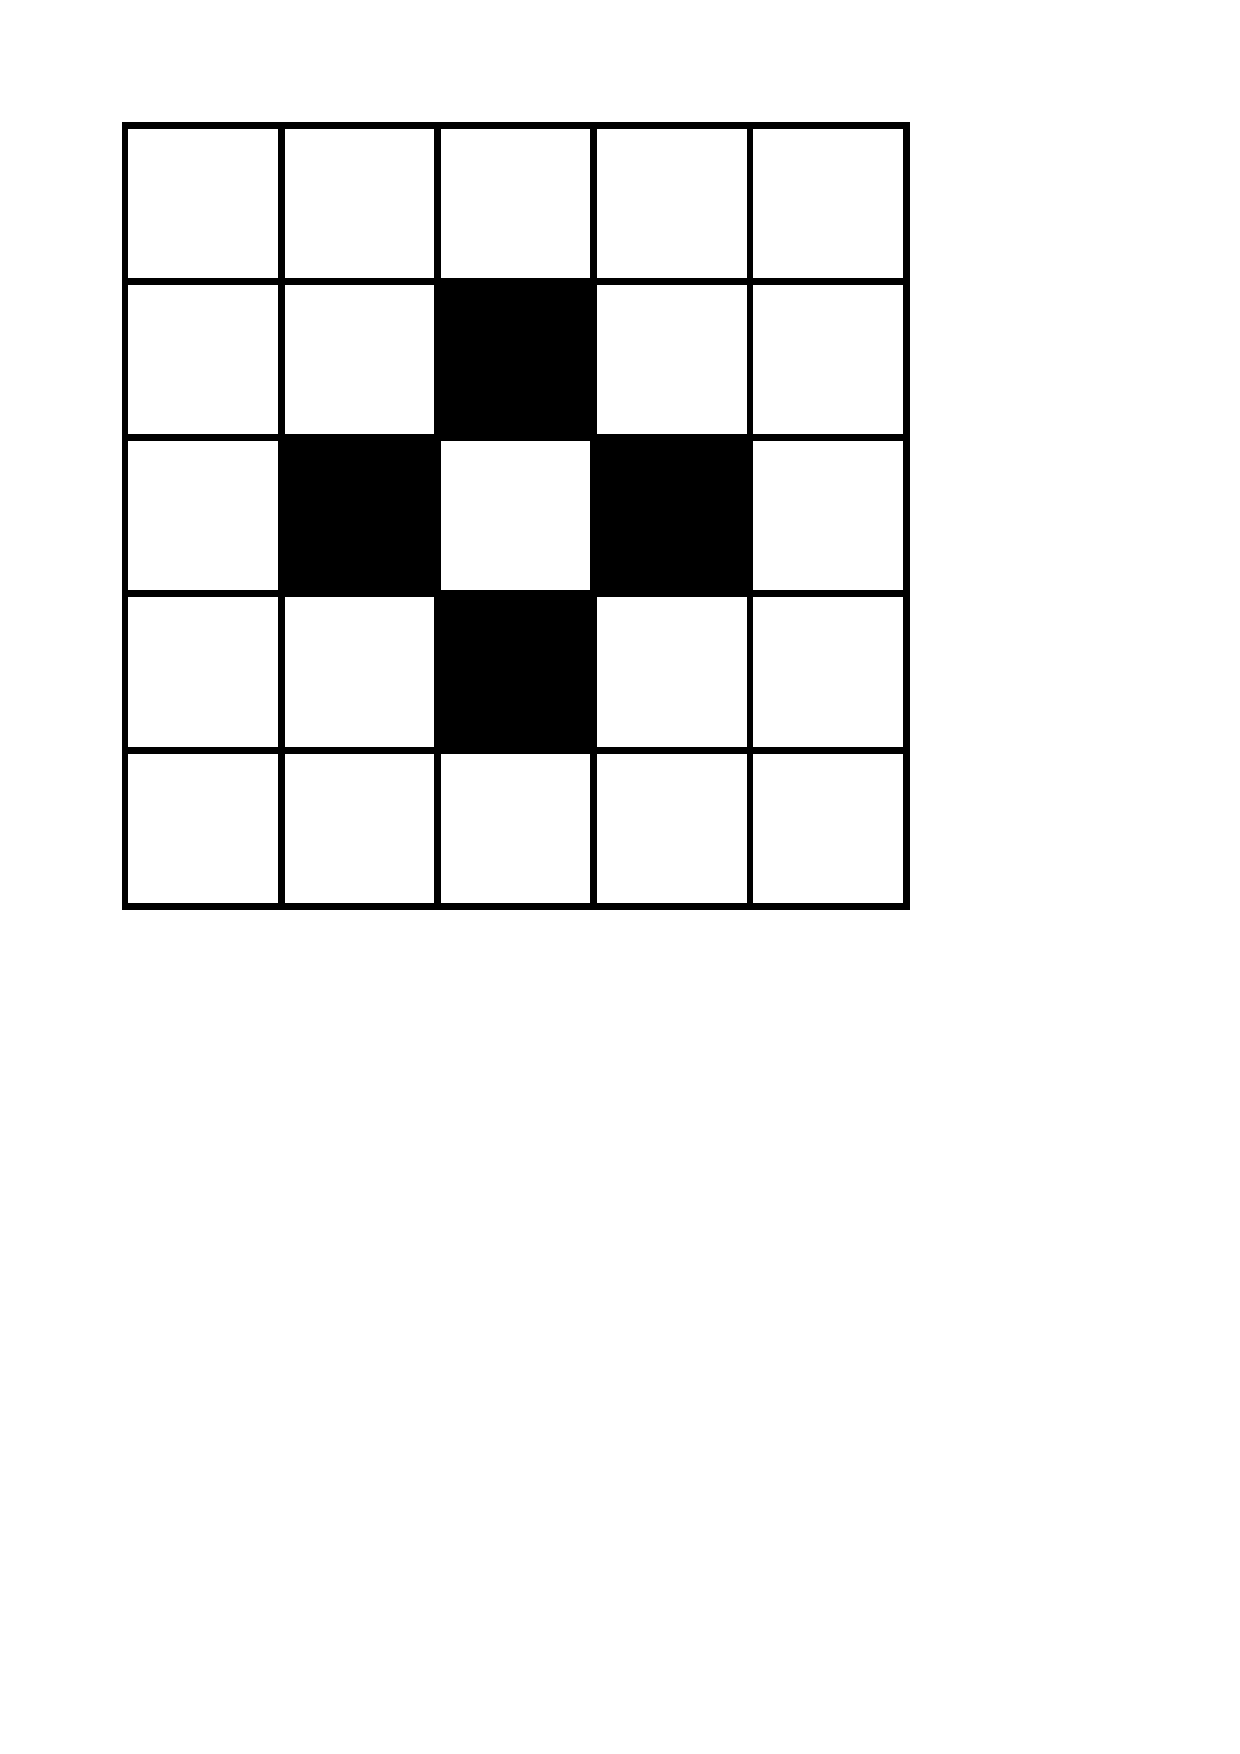
\includegraphics[width=\textwidth]{digital/4-square}
        \caption{}
          \label{fig:4-square}
        \end{subfigure}
          \hspace{.3cm}
         \begin{subfigure}[b]{0.3\textwidth}
        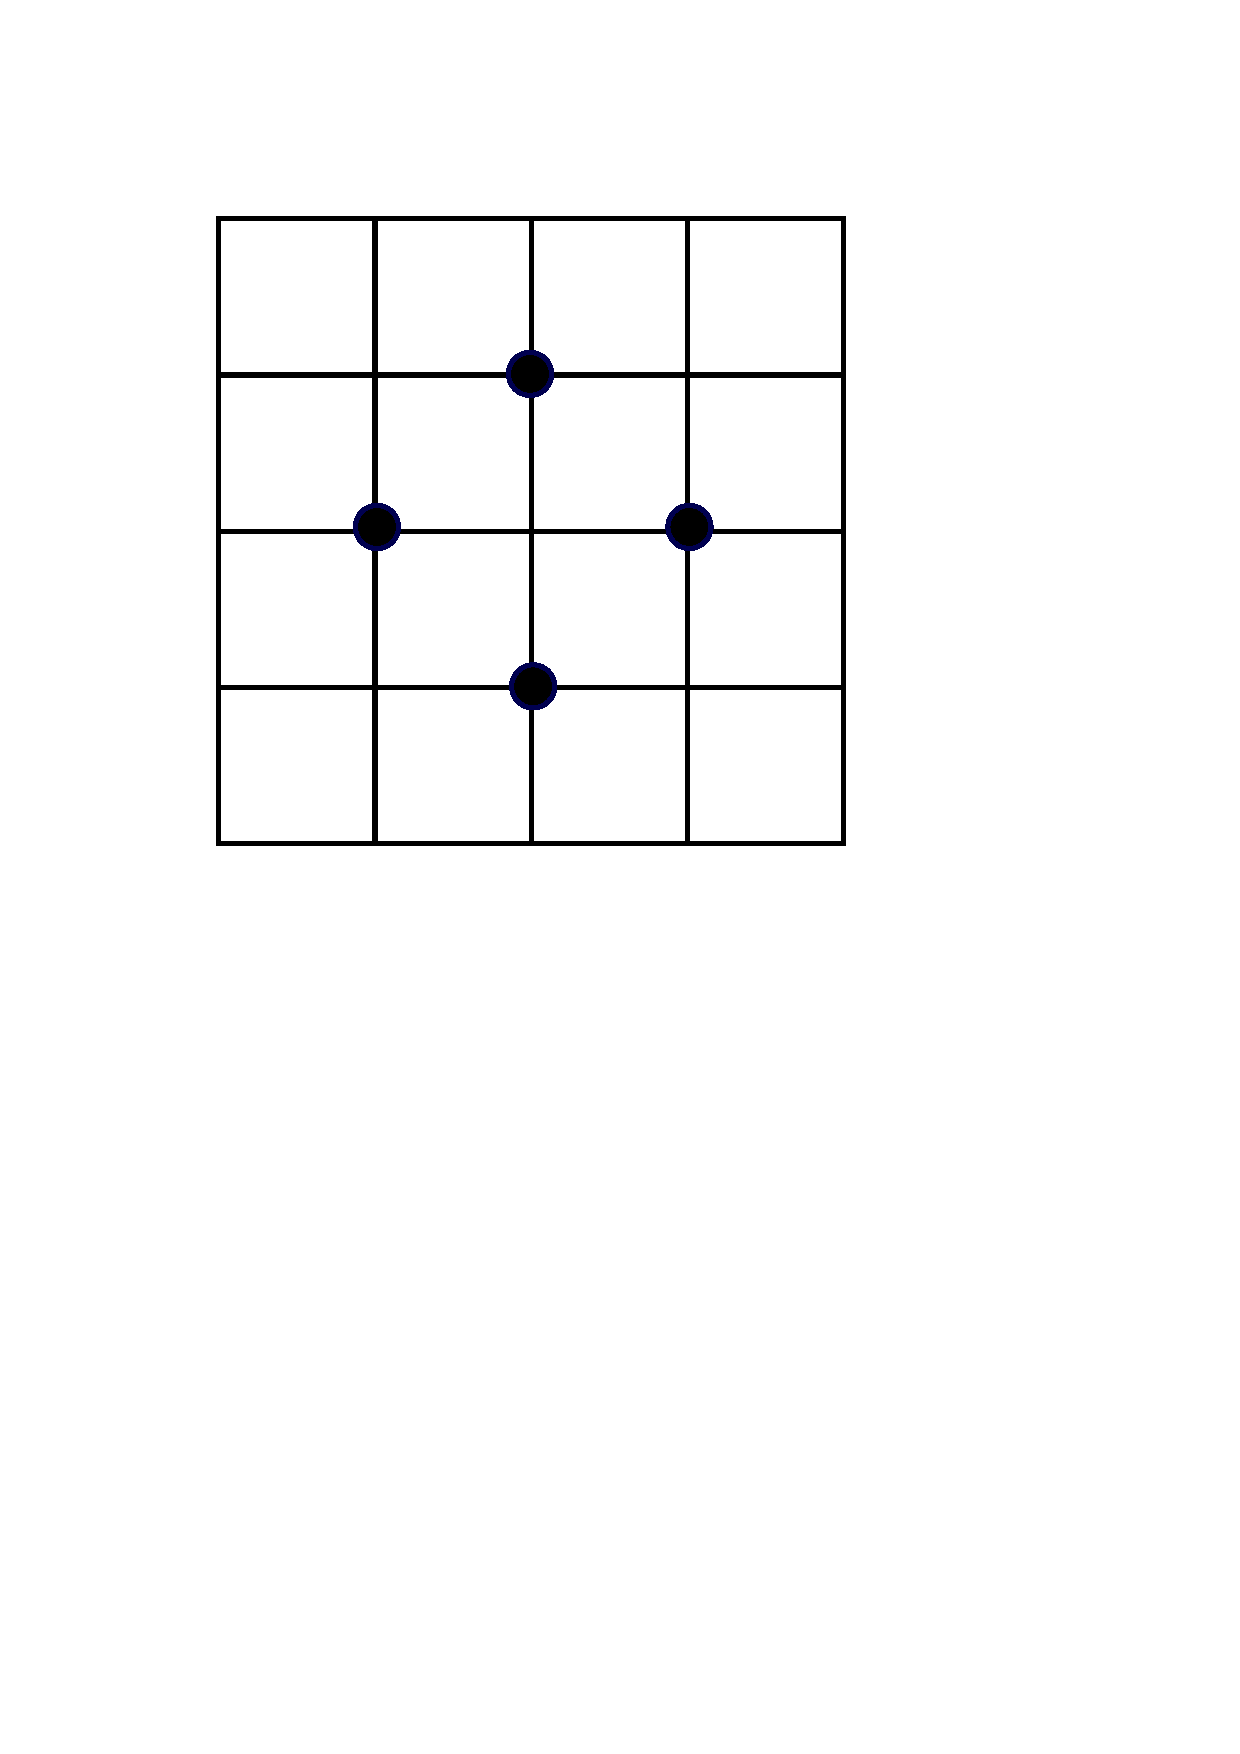
\includegraphics[width=\textwidth]{digital/4-square-dual}
        \caption{}
        \label{fig:4-square-dual}
        \end{subfigure}\\
		\caption{(\subref{fig:4-square}) A two dimensional image with four black pixels.
		Do the black pixels represent a closed curve? (\subref{fig:4-square-dual}) The same image
		represented on the lattice.
		\label{fig:4-square-and-dual}}
\end{figure}

A \EMPH{digital picture} is a quadruple $(V,m,n,B)$ where
$V=\R^2$ and $(m,n)=(4,8)$ or $V=\R^3$ and $(m,n)=(6,26)$
and $B$ is a subset of $V$. Elements of $B$ are black vertices
and elements not in $V$ are white.


One may ask, why don't we triangulate the cubical complex and
count vertices, edges, and faces to determine the genus.
One reason against doing this is that 
decomposing a cubical complex into a simplicial complex
results in 24 times as many highest dimensional cells \cite{Kaczynski2003}.


We consider cubical spaces in $\R^3$ with $(6,26)$-connectivity,
where two points are adjacent if their Euclidean distance is one.
If $M$ is a closed, orientable digital surface, there are
six types of digital surface points, these are shown in \figref{surface-points}.

\begin{figure}[htb]
        \centering
        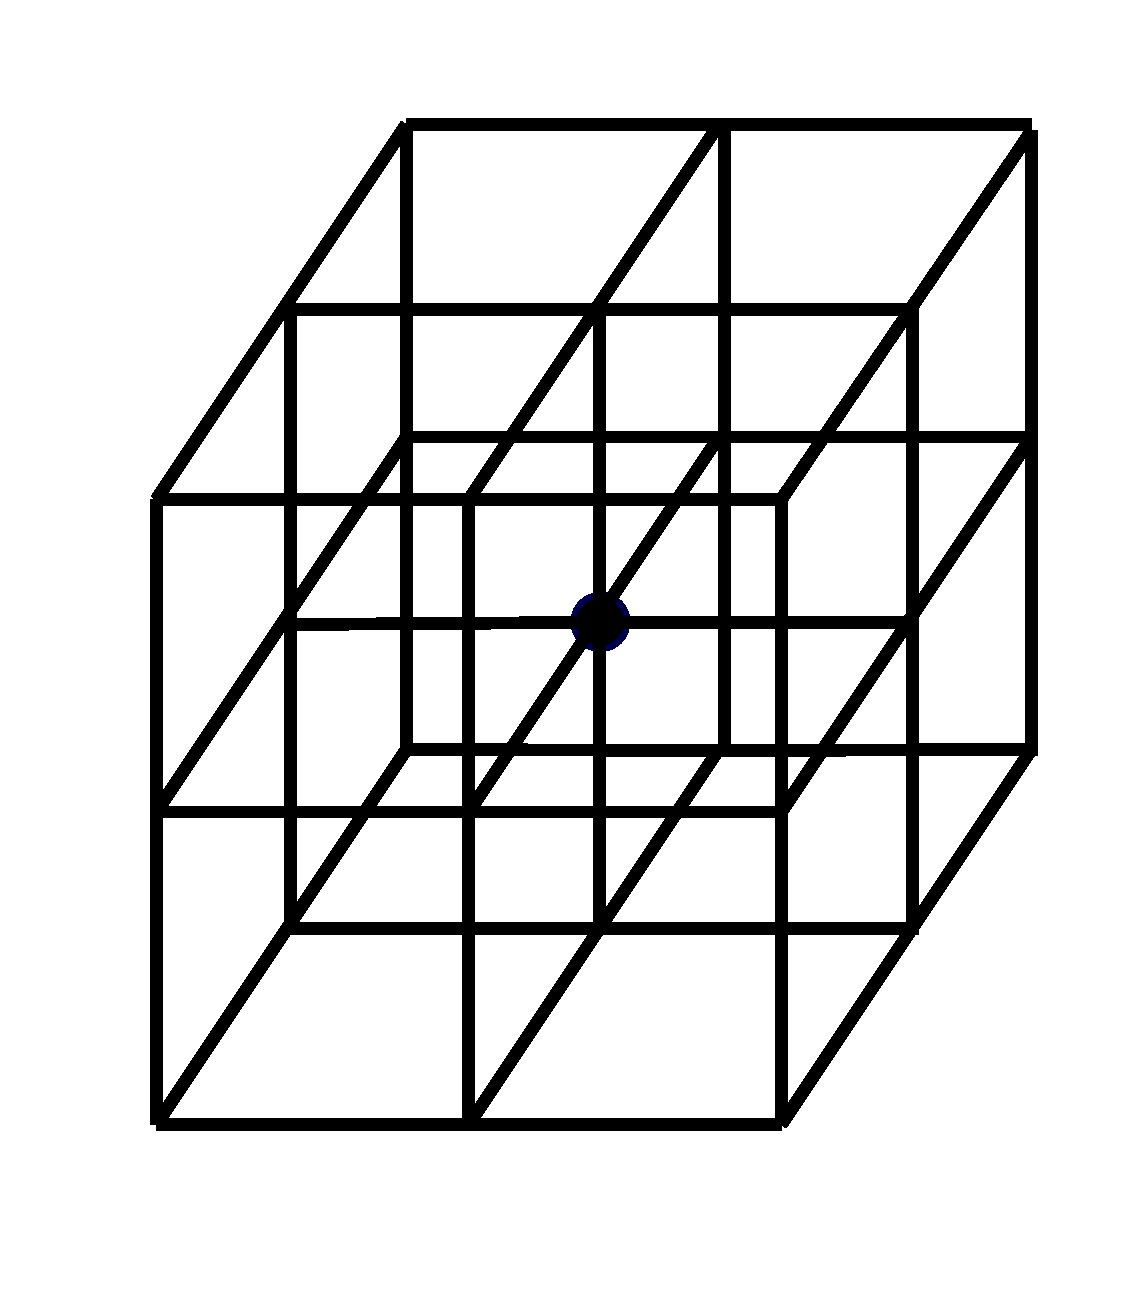
\includegraphics[width=.45\textwidth]{digital/26-neighbors}
		\caption{A vertex in a three dimensional cubical complex and its 26 neighbors.
		\label{fig:26-neighbors}}
\end{figure}


\begin{figure}[htb]
        \centering
        \begin{subfigure}[b]{0.2\textwidth}
        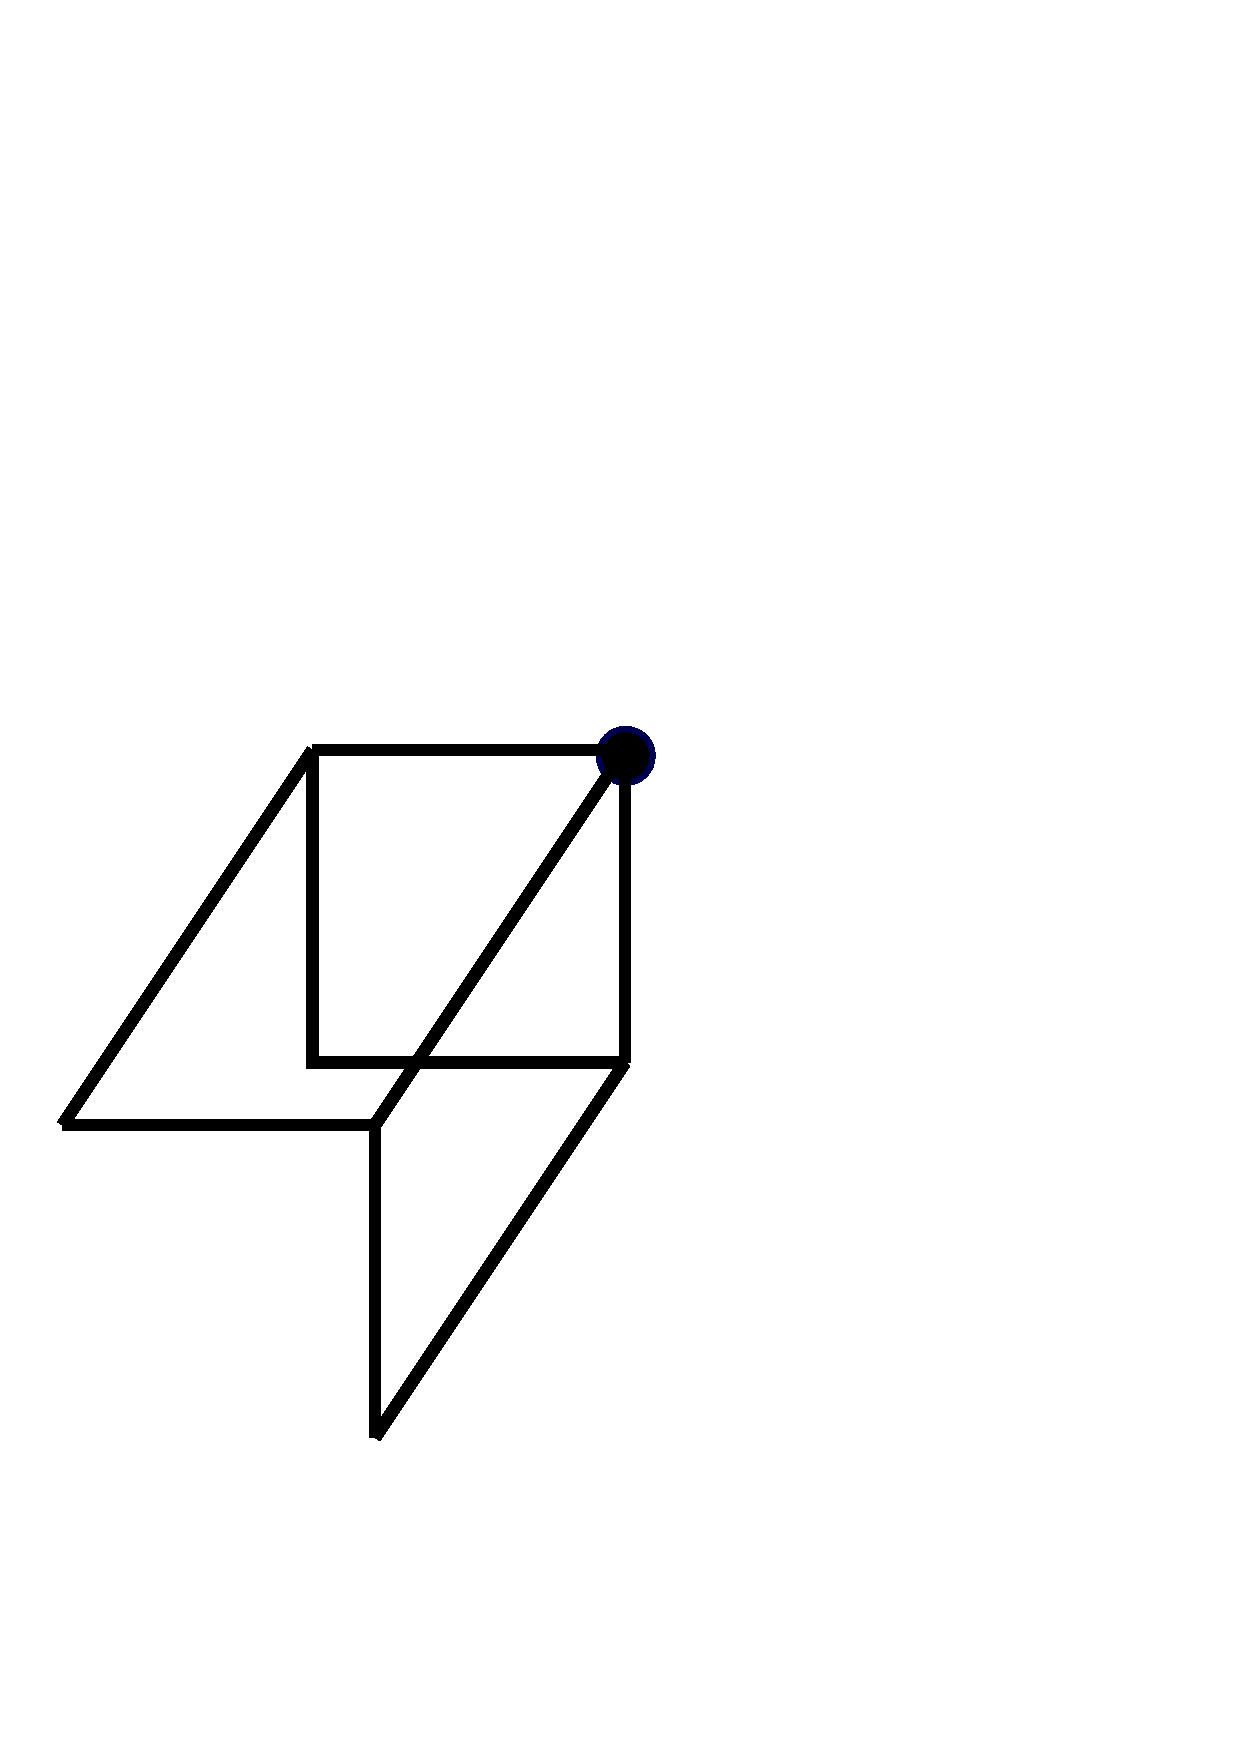
\includegraphics[width=\textwidth]{digital/3-neighbors}
        \caption{Three neighbors.}
          \label{fig:3-neighbors}
        \end{subfigure}
          \hspace{.3cm}
         \begin{subfigure}[b]{0.25\textwidth}
        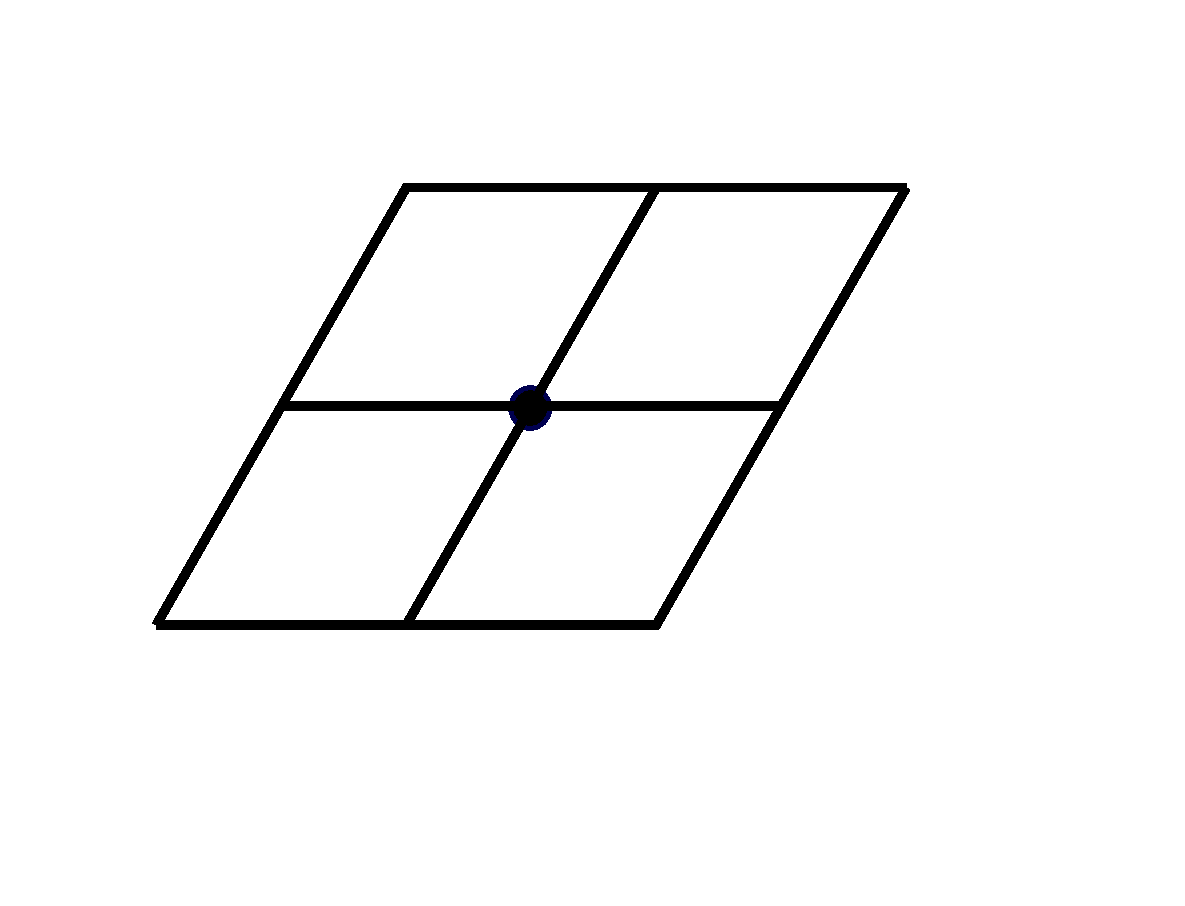
\includegraphics[width=\textwidth]{digital/4-neighbors-flat}
        \caption{Four neighbors.}
        \label{fig:4-neighbors-flat}
        \end{subfigure}
         \hspace{.3cm}
         \begin{subfigure}[b]{0.2\textwidth}
        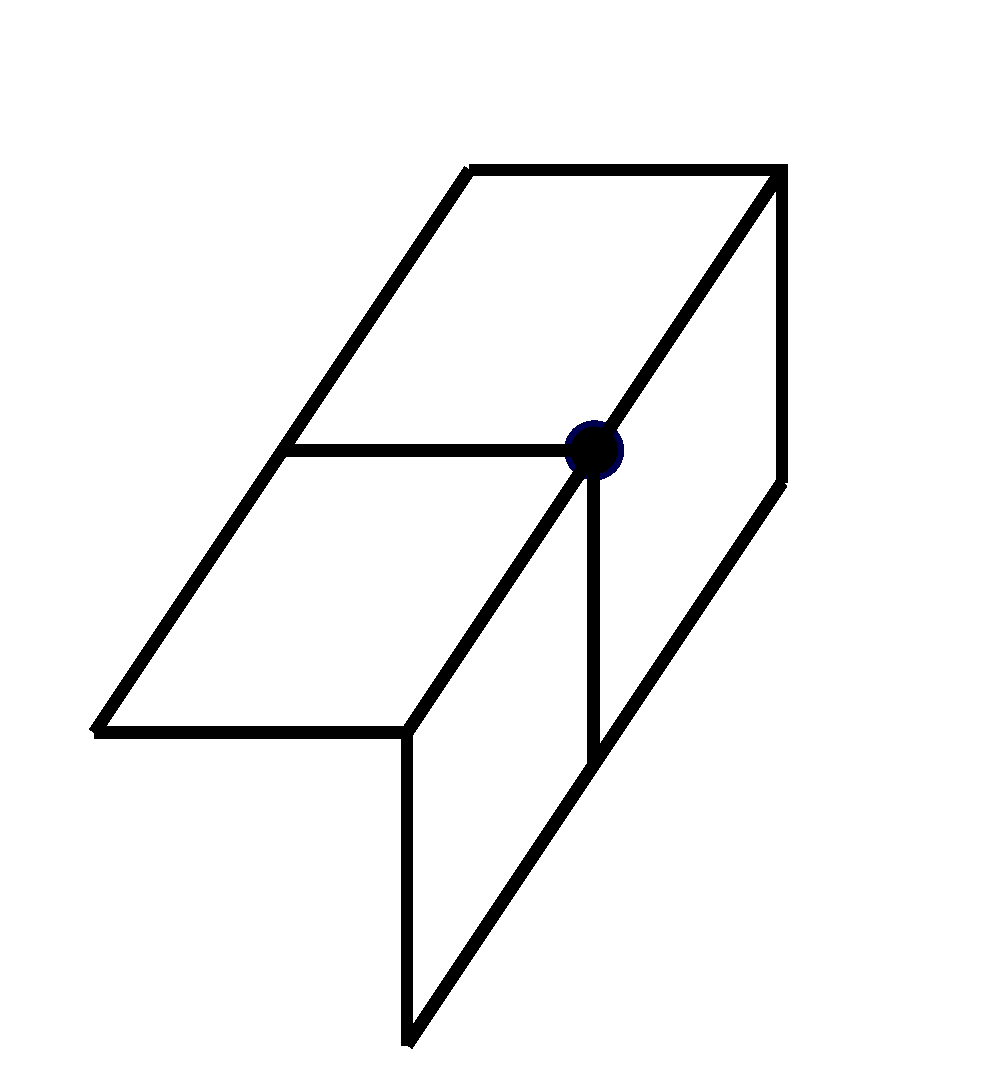
\includegraphics[width=\textwidth]{digital/4-neighbors-bent}
        \caption{Four neighbors too.}
        \label{fig:4-neighbors-bent}
        \end{subfigure}\\
         \begin{subfigure}[b]{0.25\textwidth}
        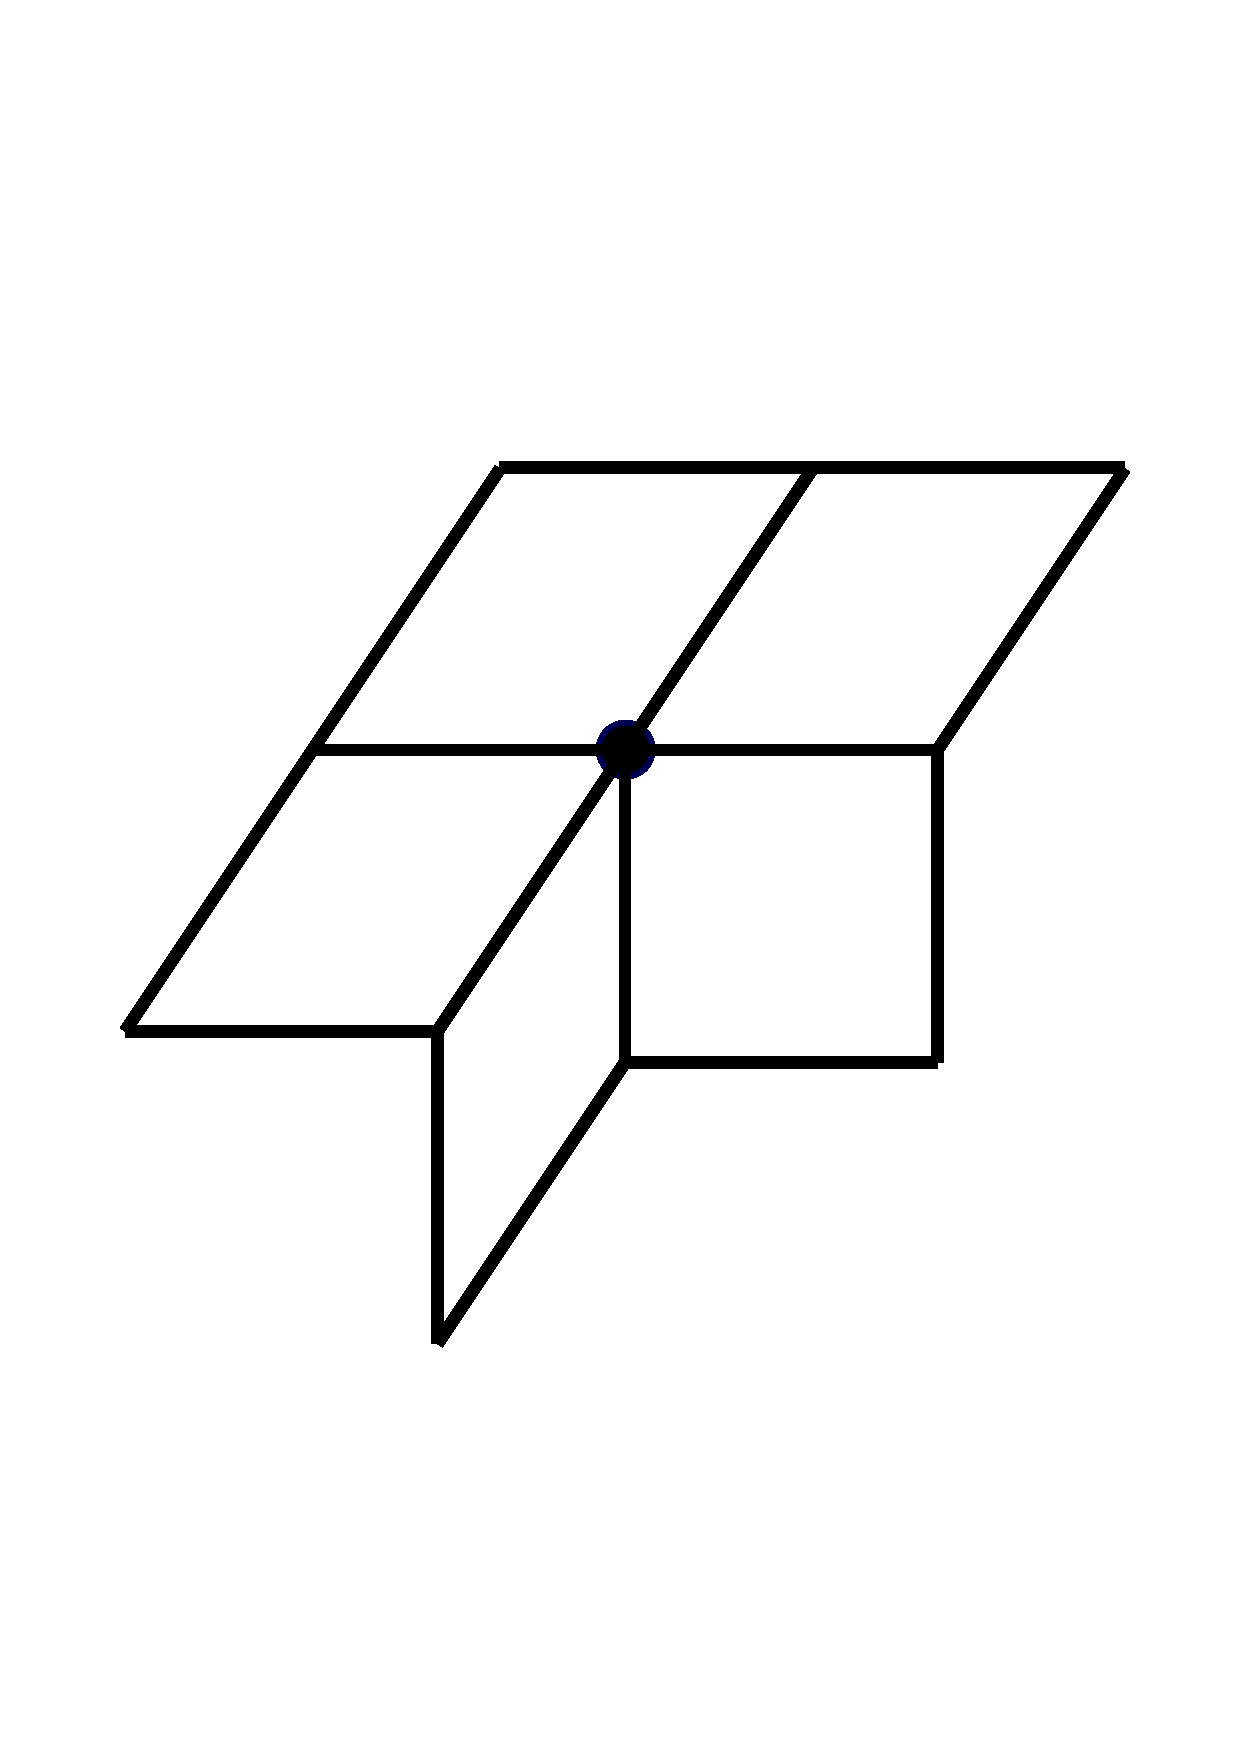
\includegraphics[width=\textwidth]{digital/5-neighbors-a}
        \caption{Five neighbors.}
          \label{fig:1-neighbors}
        \end{subfigure}
          \hspace{.2cm}
         \begin{subfigure}[b]{0.25\textwidth}
        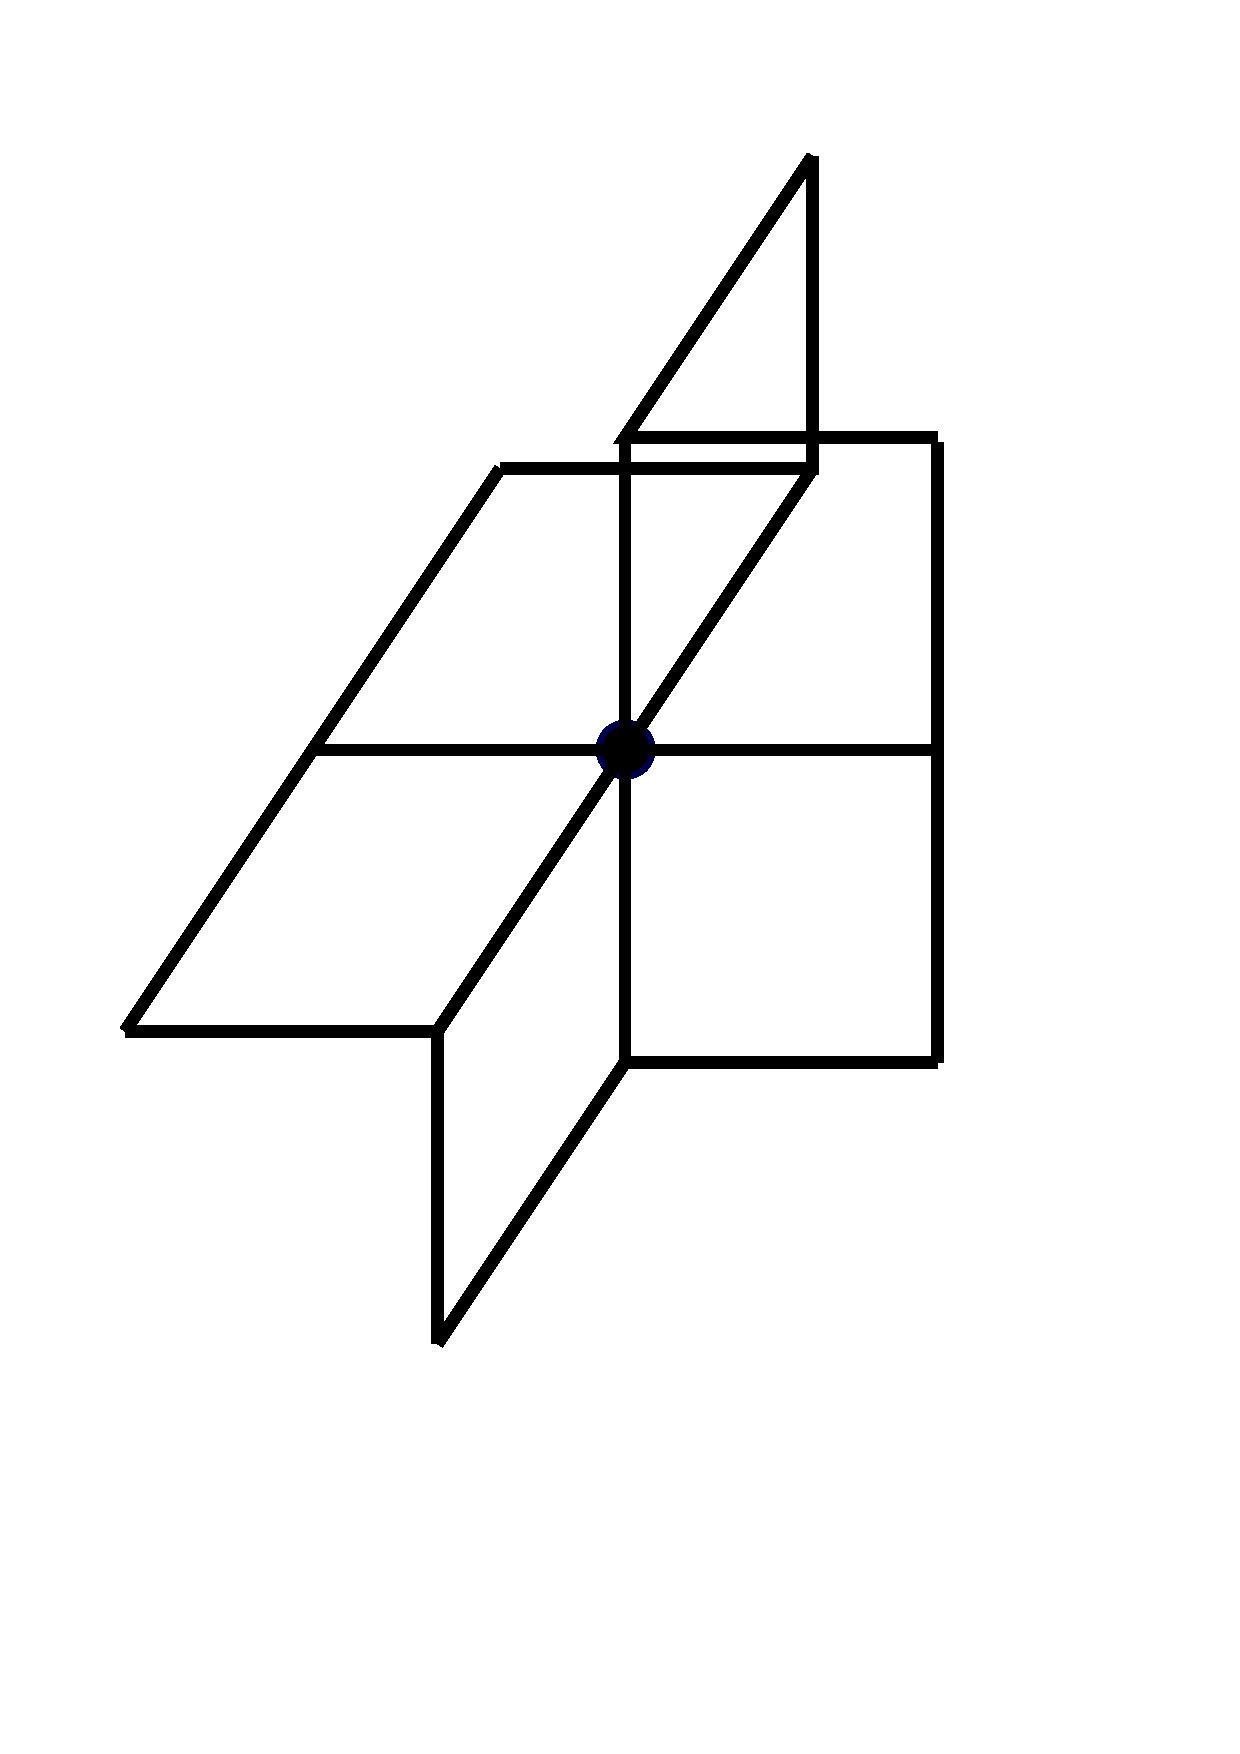
\includegraphics[width=\textwidth]{digital/5-neighbors-b}
        \caption{Six neighbors.}
        \label{fig:4-neighbors-flat}
        \end{subfigure}
         \hspace{.2cm}
         \begin{subfigure}[b]{0.25\textwidth}
        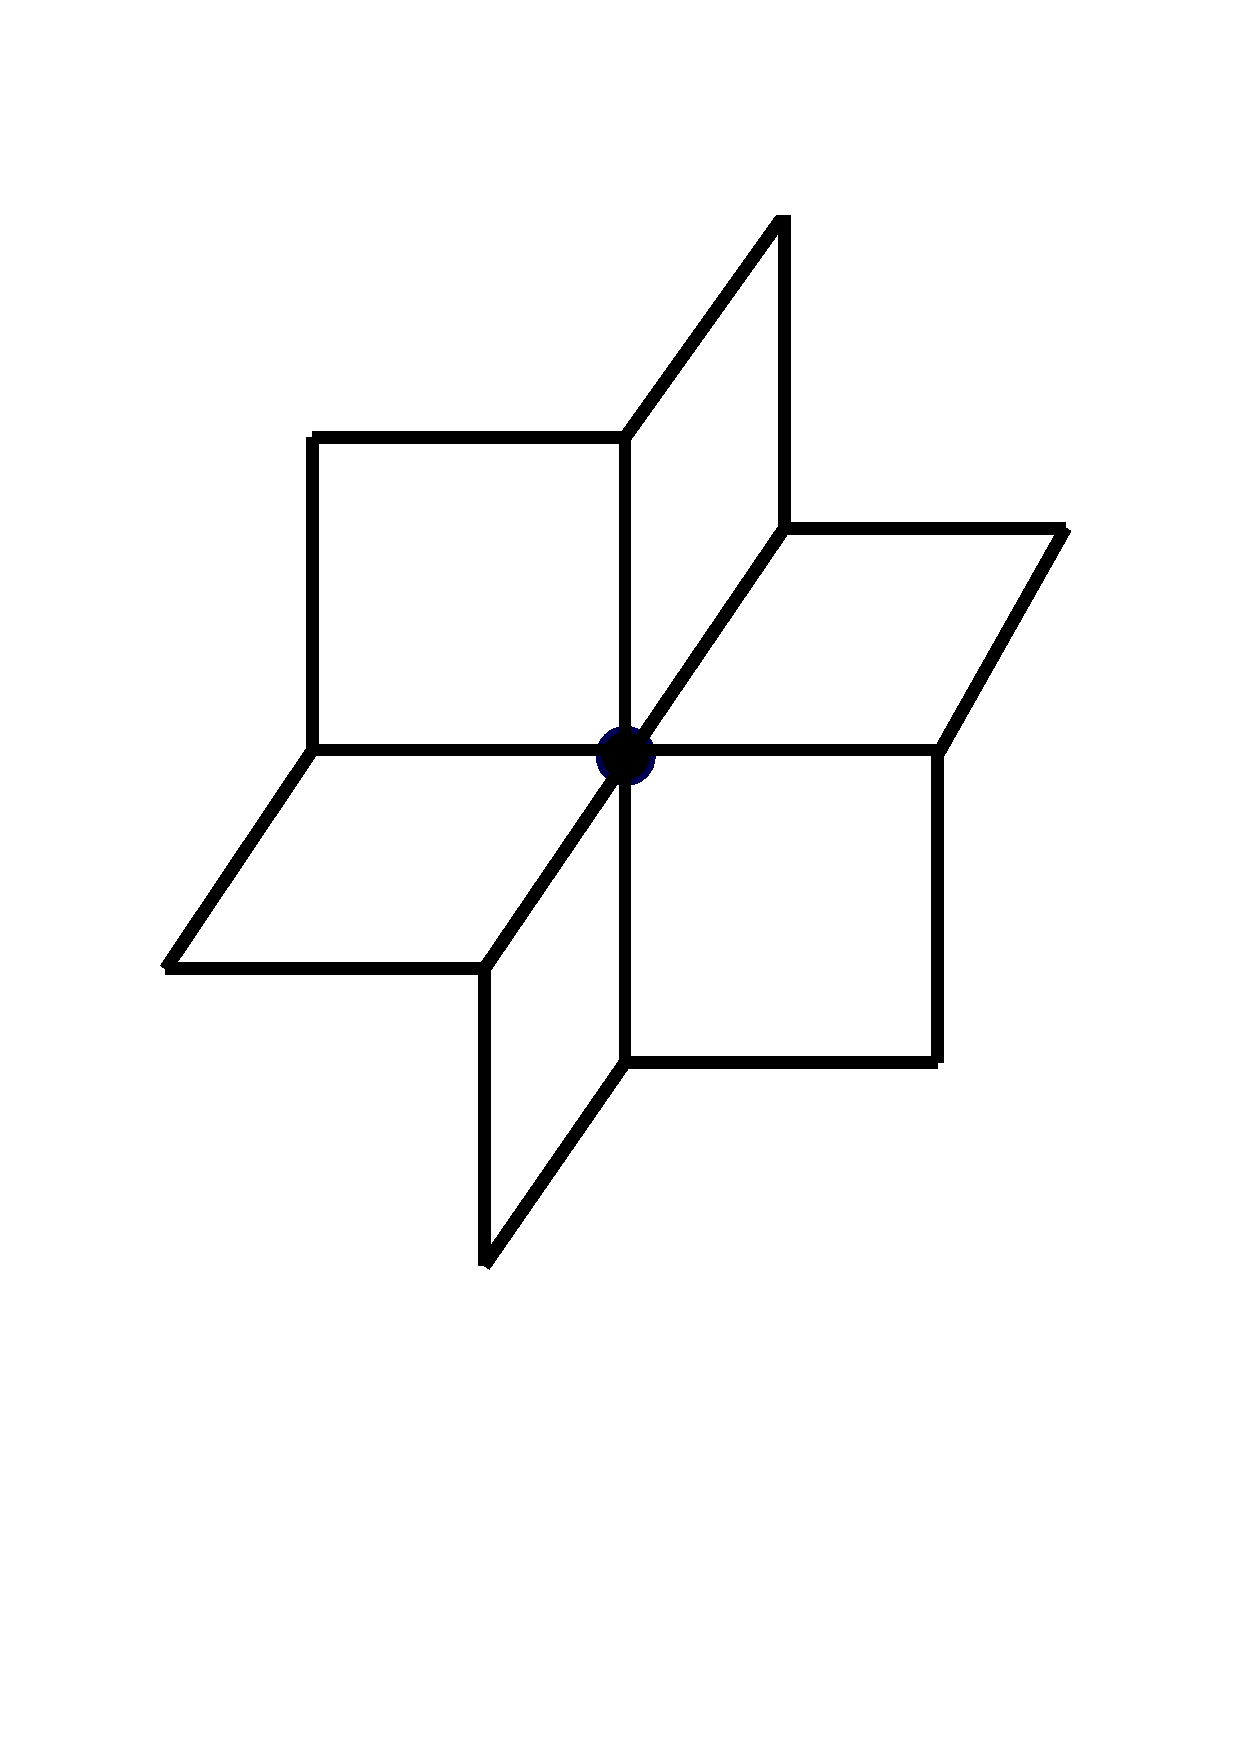
\includegraphics[width=\textwidth]{digital/6-neighbors}
        \caption{Six neighbors too.}
        \label{fig:6-neighbors}
        \end{subfigure}
		\caption{(\subref{fig:3-neighbors}) A two dimensional image with four black pixels.
		Do the black pixels represent a closed curve? (\subref{fig:4-square-dual}) The same image
		represented on the lattice.
		\label{fig:4-square-and-dual}}
\end{figure}

Let $M_i$ denote the set of digital points with $i$ neighbors and $K_i$
the curvature.
Then, by \eqnref{defect}, we have
\begin{enumerate}[(a)]
\item $K_3=\pi/2,$
\item $K_4=0,$
\item $K_5=-\pi/2,$
\item $K_6=-\pi.$
\end{enumerate}

For a closed two-manifold the is the boundary of a three-dimensional
digital image, the Gauss-Bonnet theorem implies
$$\sum_{i=3}^6K_i |M_i|=2(2-2g).$$
A linear time algorithm to compute the genus is the following.
Iterate through all points in $M$ and count the neighbors at each point
and keep track of $M_i$. Then use the above equation to  calculate the genus
using 
$$g=1+(|M_5|+2|M_6|-|M_3|)/8.$$